\chapter{Grammatiche ambigue}
\begin{theorem}
  Una grammatica $G=(T,N,P)$ è ambigua per $B\in N$ se esitono due differenti
  alberi di derivazione partendo da $B$ per la stessa stringa.
\end{theorem}

Per esempio la grammatica $1+1+1$ è ambigua a seconda delle parentesi.

\section{Soluzioni per l'ambiguità}
Per risolvere il problema dell'ambiguità si può cambiare la sintassi:
\subsection{Notazione prefissa}
\begin{lstlisting}[language=Java, caption={Notazione prefissa}]
Exp ::= Num | '+' Exp Exp | '*' Exp Exp
Num ::= '0' | '1'
\end{lstlisting}

In questo caso esiste un unico albero di derivazione per $"1 1+1*$ e le
parentesi non sono più necessarie.

\subsection{Notazione postfissa}
\begin{lstlisting}[language=Java, caption={Notazione postfissa}]
Exp ::= Num | Exp Exp '+' | Exp Exp '*'
Num ::= '0' | '1'
\end{lstlisting}

In questo caso esiste di nuovo un unico albero di derivazione e le parentesi
sono di nuovo non necessarie.
 
\subsection{Notazione funzionale}
\begin{lstlisting}[language=Java, caption={Notazione funzionale}]
Exp ::= Num | 'add' '(' Exp ',' Exp ')' | 'mul' '(' Exp ',' Exp ')'
Num ::= '0' | '1'
\end{lstlisting}

In questo esempio esiste un unico albero di derivazione per $add(1,mul(1,1)$.

\subsection{Notazione infissa}
Generalmente la notazione infissa è una soluzione più pratica.

\begin{itemize}
  \item si definiscono le regole di associatività per gli operatori binari:
    \begin{itemize}
      \item addizione associativa a sinistra: $"1+1+1"$ diventa $"(1+1)+1"$;
      \item addizione associativa a destra: $"1+1+1"$ diventa $"1+(1+1)"$;
    \end{itemize}
  \item si definiscono le regole di precedenza per gli operatori, usando
    le parentesi per sovrascriverlo:
    \begin{itemize}
      \item la moltiplicazione ha precedenza rispetto l'addizione: $"1+1*1"$
        significa $"1+(1*1)"$;
      \item l'addizione ha precedenza rispetto la moltiplicazione: $"1*1+1"$
        significa $"1*(1+1)"$.
    \end{itemize}
\end{itemize}

\subsection{Operatori con la stessa precedenza}
Gli operatori binari possono avere la stessa precedenza, in questo caso
condividono la regola associativa:
\begin{itemize}
  \item addizione e moltiplicazione hanno la stessa precedenza e sono
    associative a sinistra: $"1+1*1"$ diventa $"1+(1*1)"$ e $"1*1+1"$ diventa
    $"(1*1)+1"$;
  \item addizione e moltiplicazione hanno la stessa precedenza e sono
    associative a destra: $"1+1*1"$ diventa $"1+(1*1)"$ e $"1*1+1"$ diventa
    $"1*(1+1)"$;
\end{itemize}

\paragraph{Nota che:}
le regole sull' associatività risolvono ambiguità tra operatori binari con la
stessa precedenza, inoltre mischiando operatori con diverse \textbf{arità}
rende l'eliminazione dell'ambiguità più complessa.

\subsection{Tecniche per risolvere l'ambiguità}
\begin{itemize}
  \item una grammatica ambigua $G$ è trasformata in una grammatica non ambigua
    $G^\prime$;
  \item l' \textbf{equivalenza} significa che per tutti i non terminali di
    $B$ e $G$, i linguaggi generati da $G,G^\prime,B$ sono uguali;
  \item è possibile per la \textbf{trasformazione} di codificare l'
    associatività e le regole di precedenza nella grammatica non ambigua
    $G^\prime$.
\end{itemize}

\subsubsection{Esempio 1: + e * con la stessa precedenza}
\begin{lstlisting}[language=Java, caption={Grammatica ambigua}]
Exp ::= Num | Exp '+' Exp | Exp '*' Exp | '(' Exp ')'
Num ::= '0' | '1'
\end{lstlisting}

\begin{lstlisting}[language=Java, caption={Associatività a sinistra non ambigua}]
Exp ::= Atom | Exp '+' Atom | Exp '*' Atom
Atom ::= Num | '(' Exp ')'
Num ::= '0' | '1'
\end{lstlisting}
Nota che: $Exp '+' Atom | Exp '*' Atom$ significa che sul lato destro di
$+(*)$, le addizione (e moltiplicazioni) sono permesse solo se circondate da
parentesi.

\begin{tikzpicture}[sibling distance=10em,
  every node/.style = {shape=rectangle, rounded corners, draw, align=center}]]
  \node {exp}
    child { node {exp} 
      child { node {exp}
        child { node {atom}
          child { node {num} 
            child { node {1} }
          }
        }
      }
      child { node {+} }
      child { node {atom}
        child { node {num}
          child {node {1} }
        }
      }
    }
    child { node{*} }
    child { node{atom}
      child { node {num}
        child { node {1} }
      }
    };
\end{tikzpicture}

\begin{lstlisting}[language=Java, caption={Associatività a destra non ambigua}]
Exp ::= Atom | Atom '+' Exp | Atom '*' Exp
Atom ::= Num | '(' Exp ')'
Num ::= '0' | '1'
\end{lstlisting}
Nota che: $Atom '+' Exp | Atom '*' Exp$ significa che sul lato sinistro di 
$+(*)$,le addizione (e moltiplicazioni) sono permesse solo se circondate da
parentesi.
\begin{figure}[H]
  \centering
  \resizebox{.5\textwidth}{!}{%
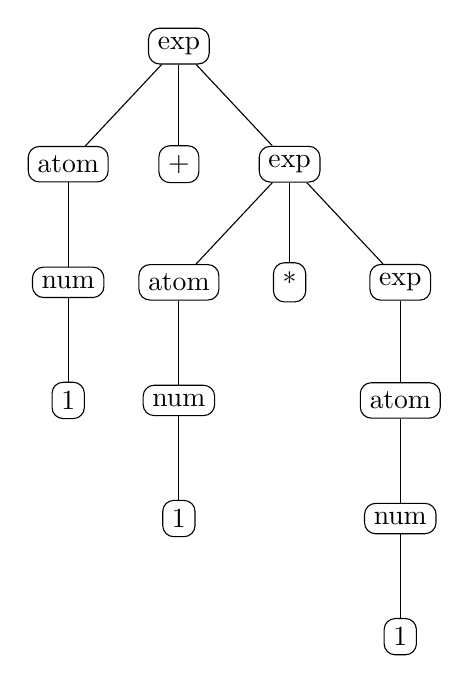
\begin{tikzpicture}[sibling distance=4em,
  every node/.style = {shape=rectangle, rounded corners, draw, align=center}]
  \node {exp}
    child { node{atom}
      child { node {num}
        child { node {1} }
      }
    }
    child { node{+} }
    child { node {exp} 
      child { node {atom}
        child { node {num}
          child {node {1} }
        }
      }
      child { node {*} }
      child { node {exp}
        child { node {atom}
          child { node {num} 
            child { node {1} }
          }
        }
      }
    };
\end{tikzpicture}
}
\end{figure}

\subsubsection{Esempio 2: * con la maggiore precedenza}
\begin{lstlisting}[language=Java, caption={Associative a sinistra non ambigue}]
Exp ::= Mul | Exp '+' Mul
Mul ::= Atom | Mul '*' Atom'
Atom ::=  Num | '(' Exp ')'
Num ::= '0' | '1'
\end{lstlisting}
Nota che: $Mul '*' Atom $ significa che entrambi i lati delle addizione di $*$
sono permesse solo se circondate da parentesi.

\begin{lstlisting}[language=Java, caption={Associative a destra non ambigue}]
Exp ::= Mul | Exp '+' Mul
Mul ::= Atom | Atom '*' Mul'
Atom ::=  Num | '(' Exp ')'
Num ::= '0' | '1'
\end{lstlisting}
Nota che: $Atom '*' Mul $ significa che entrambi i lati delle addizione di $*$
sono permesse solo se circondate da parentesi.

\subsubsection{Esempi rimanenti}
\begin{itemize}
  \item $*$ con precedenza ed associativtà  a sinistra, $+$ associatività a
    destra;
  \item $*$ con precedenza ed associativtà  a destra, $+$ associatività a
    sinistra;
  \item $+$ con precedenza ed associativtà  a sinistra, $*$ associatività a
    destra;
  \item $+$ con precedenza ed associativtà  a destra, $+$ associatività a
    sinsitra;
\end{itemize}

\section{Sintassi ambigua per statements}
\begin{lstlisting}[language=Java, caption={Esempio di ambiguità per gli statements}]
Stmt ::= ID '=' Exp | 'if' '(' Exp ')' Stmt | Stmt ';' Stmt | '{' Stmt '}'
Exp ::= ID | BOOL // ID e BOOL sono definiti da espressioni regolari
\end{lstlisting}

\begin{figure}[H]
  \caption{Primo esempio di albero di derivazione per "if(x) x=false;y=true"}
  \centering\resizebox{\textwidth}{!}{%
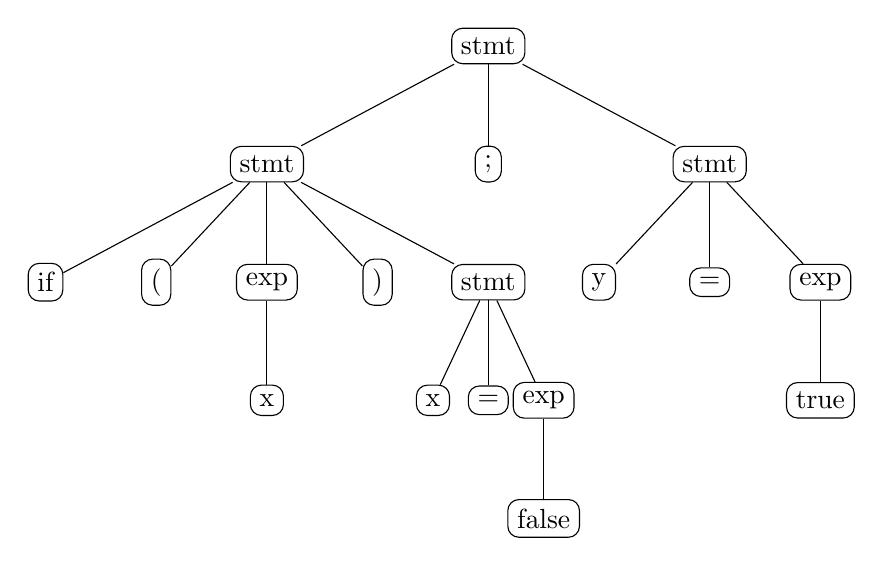
\begin{tikzpicture}[
  level 1/.style = {sibling distance=8em},   % <-- added
  level 2/.style = {sibling distance=4em},    % <-- added
  level 3/.style = {sibling distance=2em},    % <-- added
  every node/.style = {
    shape=rectangle,
    rounded corners,
    draw,
    align=center
  }]
  \node {stmt}
    child { node {stmt}
      child { node {if} }
      child { node {$($} }
      child { node {exp}
        child { node {x} }
      }
      child { node {$)$} }
      child { node {stmt}
        child { node {x}}
        child { node {=} }
        child { node {exp}
          child { node {false} }
        }
      }
    }
    child { node {;} }
    child { node {stmt}
      child { node {y} }
      child { node {=} }
      child { node {exp}
        child { node {true} }
      }
    };
\end{tikzpicture}}\end{figure}
\begin{figure}[H]
  \caption{Secondo esempio di albero di derivazione per "if(x) x=false;y=true"}
  \centering\resizebox{\textwidth}{!}{%
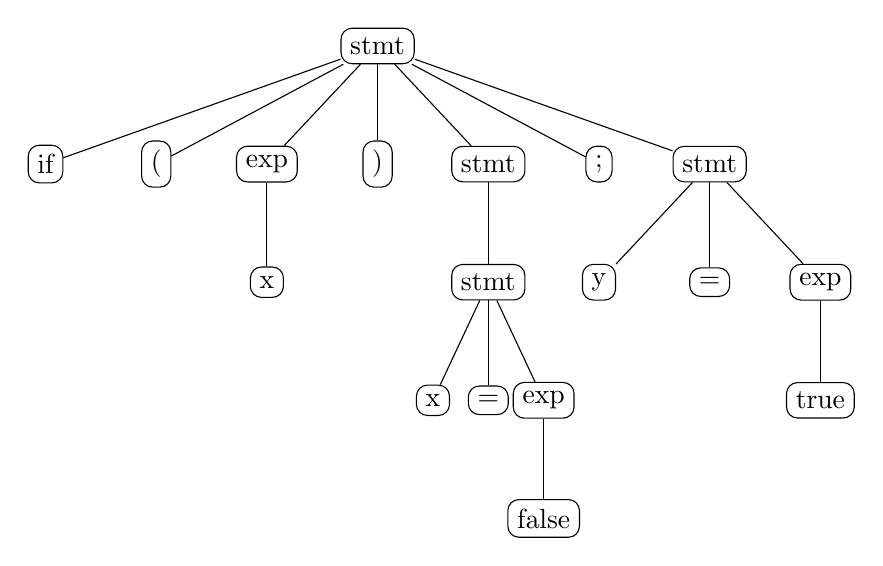
\begin{tikzpicture}[
  level 1/.style = {sibling distance=4em},   % <-- added
  level 2/.style = {sibling distance=4em},    % <-- added
  level 3/.style = {sibling distance=2em},    % <-- added
  every node/.style = {
    shape=rectangle,
    rounded corners,
    draw,
    align=center
  }]
  \node {stmt}
    child { node {if} }
    child { node {$($} }
    child { node {exp}
      child { node {x} }
    }
    child { node {$)$} }
    child { node {stmt}
      child { node {stmt}
        child { node {x} }
        child { node {=} }
        child { node {exp}
          child { node {false} }
        }
      }
    }
    child { node {;} }
    child { node {stmt}
      child { node {y} }
      child { node {=} }
      child { node {exp}
        child { node {true} }
      }
    };
\end{tikzpicture}}\end{figure}
